\documentclass[11pt]{article}

\title{Using SAS and the SAS windowing environment}
\author{}
\date{}

\usepackage{graphicx}

\begin{document}
\maketitle

\section{Introduction}
\label{sec:intro}

This is not a mathematical course, but it does involve
computing. Specifically, we will be using the statistical package SAS:
learning how to analyze data using the methods we learn, and how to
interpret the output.

SAS has been around for years (now on version 9), and has become the
standard in industry, government and suchlike places for "routine"
statistical analysis (that is, where more or less well-known
statistical procedures are to be used). If you can say, therefore,
that you have experience with SAS, it makes you that much more
employable! SAS runs on Windows, Unix, the Mac, etc; it is big, and
expensive, but there are certain common themes, and, as we will see,
once you see how to run one analysis, you can easily learn how to run
another. SAS is not point-and-click: you write a "program" and then
run it, but you then have the advantage of knowing exactly what you
did, and being able to run the program again, or modify it. Is SAS
user-friendly? No. But SAS, as we run it, looks exactly the same in
every environment: Windows, Unix, running on your machine or some
remote machine. So what you learn here will definitely be transferrable to
what you might see later.

SAS can be run in two ways: a ``batch mode'',
and a windowing or development environment that looks nicer. The
windowing environment also makes it possible to get nicer plots.

\section{Setup}

If you happen to be running Linux (or a Mac), 
there's no setup required, beyond being able to open a terminal
(command-line) window. Go straight to the next section.

In the likelier event that you're running Windows, you have a couple
of things to organize first. 

First you need a program called \verb-Xming- that allows SAS's
windowing environment to happen in Windows (even though Mathlab runs
Ubuntu Linux). Download this from
\verb-sourceforge.net/projects/xming-, clicking on the big green
button, and install it in the usual way. Allow it to place a shortcut
on your desktop for ease of use later.

Then you need a program called \verb-putty-, which you can get from
\verb-putty.org-. This actually enables you to connect to
Mathlab. Just download \verb-putty.exe- and save it on your desktop
--- there's no install required. (Choose ``save'' rather than ``run''
to download it.)

To test your installation, first run Xming by double-clicking on its
icon. This will appear to do nothing except put a big X in your system
tray. Now start Putty as well (ignoring any ``unknown publisher''
warnings). There are a few things to enter before you can connect to
Mathlab. In the Host name box, enter
\verb-mathlab.utsc.utoronto.ca-. Leave Port 22 and Connection Type SSH
as they are. Then in the Category window on the left, look for SSH
with a plus sign next to it (down near the bottom). Click on the plus
sign. Look for X11 in the choices that pop out (the fourth one). Click
on it. On the right there is ``Enable X11 forwarding'' with a check
box next to it. Click on the check box. Then look in the Category
window on the left for Session (right at the top) and click on
it. This takes you back to where you started. Save this (so you don't
have to do it every time) by first typing a name like \verb-mathlab-
into the Saved Sessions box, and then clicking on the Save button on
the right. The name you chose appears in the bottom box below Default
Settings.

Now you can get connected. In Putty, click Open. This will bring up a
black screen asking for your Mathlab username and password (the same
as your UTSCid ones). If you can't log in, check your password, and if
you still can't, let me know. If you can, you'll see some stuff
including ``Ubuntu comes with ABSOLUTELY NO WARRANTY'', and then it
waits for you to type something. Type \verb-sas-, and you should
(eventually) see a splash screen and a whole bunch of windows appear,
including SAS Explorer, SAS Log and SAS Program Editor. (If you get
some kind of error message, check that you do have Xming running.)
If you want to
explore further, you can, but this is enough to show that you have SAS
running. To exit, go to SAS Explorer's File menu, select Exit, and
then confirm this in the dialog box that follows.

\section{Starting SAS}
\label{sec:runsas}

On Linux or a Mac,
open up a terminal window and type

\begin{verbatim}
ssh -X username@mathlab.utsc.utoronto.ca
\end{verbatim}

where you replace \verb-username- with your actual UTSC
username. Jump over the next paragraph, and ignore anything about Xming.

On Windows, start up Xming, then run Putty, loading your saved
\verb-mathlab- profile (click on \verb-mathlab-, then click
Load). Click Open to connect. Enter your username (UTSCid) when
prompted.

Then enter your password (the one that goes with your UTSCid). If it
doesn't work, check it and try again; if it still doesn't work, ask
me.

You'll see a whole bunch of things indicating that you are connected
to Mathlab. At the command prompt type \verb-sas-, and in due course a
whole bunch of windows will appear with names like SAS Explorer, SAS
Log and SAS Program Editor. If typing SAS gets you an error, the
likely cause is that you forgot to start Xming first.


\section{Using SAS}
\label{UsingSAS}

From here on, it's the same whatever system you are running, or
whatever machine you are running SAS on. (If you happen to have SAS
installed on your own machine, it looks exactly the same.)

To give SAS something to work on, find the Program Editor window (with
a list of line numbers down the left side). This works something like
most editors you may have seen, with a couple of non-intuitive
features. First off, the program editor's default is ``overwrite
mode'', where anything you type overwrites anything that was there
before. Most editors you know probably use ``insert mode''; to switch
to insert mode here, press the ``insert'' key, and now any text you
already typed will get shunted to the right when you type in something
new.

The URL

\begin{verbatim}
http://tinyurl.com/sas-editor
\end{verbatim}

redirects to the SAS support page on using the program editor. (The
original URL is rather imposingly long.)

As an example, type the below (with the semicolons exactly as shown) into
the Program Editor. (Confusingly, hitting Enter at the end of a line
doesn't insert a new line, even in insert mode. To insert a new line,
go back onto the line numbers, type ``i'' and Enter, and a blank line
will be inserted below where you typed the ``i''.)

\filbreak
\begin{verbatim}
data x;
  input x;
  cards;
1
2
3
5
7
;

proc print;

proc means;

run;
\end{verbatim}
\filbreak

This means the following:

\begin{itemize}
\item Here comes a data set called \verb-x-, with one variable, also
  called \verb-x-.
\item Here come the data values. (You can use \verb-datalines- instead
  of \verb-cards-, but I like the throwback to the days of punched cards.)
\item The five values for \verb-x- are 1,2,3,5 and 7.
\item \verb-proc print- just lists the data, so you can check that the
  values were read in properly.
\item \verb-proc means- calculates means and SDs for all the variables
  (just \verb-x-, here).
\end{itemize}

Once you have this right to your satisfaction, see whether it works by
either: finding the SAS Toolbar and clicking on the running human over
to the right, or clicking on the Run Menu in the Program Editor and
selecting Submit. This (rather worryingly) makes your
painstakingly-typed SAS commands disappear (don't worry, you can get
them back) and runs SAS on them. If everything (or even something) is
OK, the Output window will pop up, and you will see your results (use
Page Up to see previous pages); if not (for example, you see some of
what you were expecting but not all), find the Log window, and look
for any errors there. I mistakenly typed \verb-proc mean- as
\verb-proc meanbubbles-, and got an output window with just the output
from \verb-proc print- in it, and this in the Log window:

\filbreak
\begin{verbatim}
1    data x;
2      input x;
3      cards;

NOTE: The data set WORK.X has 5 observations and 1 variables.
NOTE: DATA statement used (Total process time):
      real time           0.46 seconds
      cpu time            0.01 seconds


9    ;
10
11   proc print;
12

NOTE: There were 5 observations read from the data set WORK.X.
NOTE: PROCEDURE PRINT used (Total process time):
      real time           0.20 seconds
      cpu time            0.05 seconds


13   proc meanbubbles;
ERROR: Procedure MEANBUBBLES not found.
14
15   run;

NOTE: The SAS System stopped processing this step because of errors.
NOTE: PROCEDURE MEANBUBBLES used (Total process time):
      real time           0.05 seconds
      cpu time            0.00 seconds

\end{verbatim}
\filbreak

This all means:

\begin{itemize}
\item The data were read in properly (there should be 5 observations
  on 1 variable).
\item \verb-proc print- worked just fine (no errors) and any output
  from it will appear in the Output window.
\item \verb-proc meanbubbles- does not exist, so SAS can't run
  it. This is (predictably) an Error.
\end{itemize}

To get your commands back, bring up the Program Editor window, click
on Run, and select Recall Last Submit. Go down to line 13 (the line
with \verb-proc meanbubbles- on it), and change it to the correct
\verb-proc means-. (You might need to use Page Down rather than the
cursor down key to get to this line.)

The output looks like this:

\filbreak
{\footnotesize
\begin{verbatim}
                                           The SAS System         09:57 Monday, January 10, 2011   2

                                              Obs    x

                                               1     1
                                               2     2
                                               3     3
                                               4     5
                                               5     7
\end{verbatim}
}
\filbreak

which is the output of \verb-proc print-, and on the next page:

\filbreak
{\footnotesize
\begin{verbatim}
                                           The SAS System         09:57 Monday, January 10, 2011   3

                                        The MEANS Procedure

                                       Analysis Variable : x

                 N            Mean         Std Dev         Minimum         Maximum
                 -----------------------------------------------------------------
                 5       3.6000000       2.4083189       1.0000000       7.0000000
                 -----------------------------------------------------------------
\end{verbatim}
}
\filbreak

\verb-proc print- confirms that the data were read in correctly, while
\verb-proc means- actually tells us something interesting about the data.

You see that the output is rather wide, and needs to be shrunk quite a
bit to get it on the page. You can change this by going to the SAS
Explorer window, selecting Tools, Options and System (in order), clicking the
plus sign next to Log and Procedure Output Control, then clicking on
SAS log and procedure output. Not exactly easy to find. In the
right-hand part of the window, find Linesize (by default 100) and {\em
  right}-click on it to change it to something like 80.

Go back to the Program Editor, recall the commands you just submitted
(Run and Recall Last Submit), and then submit them again. The output
from \verb-proc means- now looks like this:

\filbreak
{\small
\begin{verbatim}
                                 The SAS System                                5
                                                  09:57 Monday, January 10, 2011

                              The MEANS Procedure

                             Analysis Variable : x

       N            Mean         Std Dev         Minimum         Maximum
       -----------------------------------------------------------------
       5       3.6000000       2.4083189       1.0000000       7.0000000
       -----------------------------------------------------------------
\end{verbatim}
}
\filbreak

which required a good bit less shrinking to get it onto the page.

\section{Saving and opening}

This is a good place to mention that you can save your commands (and
embedded data) should you wish to use them again later. Recall the commands
into the Program Editor, then select Save or Save As from the Program
Editor's File Menu. This will enable you to put them in a file {\em on
  the Mathlab machine}. By tradition, the file uses a \verb-.sas-
extension. I called mine \verb-testing.sas-. Likewise, you can re-open
a file of commands. If the Program Editor has anything in it, you'll
probably want to clear it first (SAS by default adds any read-in lines
to the end of the code that's already there) by selecting Edit and
Clear All. Then you can open a file of commands in the way you'd
guess: File and Open. You can open, edit and re-save something other
than commands by looking at the bottom of the Open dialog box for File
Type, and changing it to All Files.

Rather than embedding your data into your programming code, you can
also save your data into a file. One way to do this is to type your
data into the (empty) Program Editor and then save it into a file on
Mathlab, traditionally with the extension \verb-.dat-. The data layout
(unless you are prepared to go through some contortions in SAS) is one
observation per line, with values for all the variables separated by
whitespace. The data below are values of a response variable $y$ from
three groups labelled a, b, and c:

\filbreak
\begin{verbatim}
a 20
a 21
a 16
b 11
b 14
b 17
b 15
c 13
c 9
c 12
c 13
\end{verbatim}
\filbreak

You can type these, one per line, into the Program Editor, and then
save everything in a file called \verb-threegroups.dat-. Then you can
clear the Program Editor window (Edit, Clear All: don't try to submit
these lines!) and type the following program:

\filbreak
\begin{verbatim}
data groups;
  infile 'threegroups.dat';
  input group $ y;

proc print;

proc means;
  class group;
  var y;

run;
\end{verbatim}
\filbreak

Note that the filename has {\em single} quotes around it. This a bit
cleaner than the code with \verb-cards- (or \verb-datalines-) and the
actual data in it, because you can see rather more clearly what's
going on. Running this produces no errors (check the Log window to be
sure) and two pages of output. The first just lists the data, like
this:

\filbreak
{\small
\begin{verbatim}
                                 The SAS System                                6
                                                  09:57 Monday, January 10, 2011

                               Obs    group     y

                                 1      a      20
                                 2      a      21
                                 3      a      16
                                 4      b      11
                                 5      b      14
                                 6      b      17
                                 7      b      15
                                 8      c      13
                                 9      c       9
                                10      c      12
                                11      c      13
\end{verbatim}
}
\filbreak

and the second shows the means for each group separately:

\filbreak
{\small
\begin{verbatim}
                                 The SAS System                                7
                                                  09:57 Monday, January 10, 2011

                              The MEANS Procedure

                            Analysis Variable : y

             N
group      Obs    N           Mean        Std Dev        Minimum        Maximum
-------------------------------------------------------------------------------
a            3    3     19.0000000      2.6457513     16.0000000     21.0000000

b            4    4     14.2500000      2.5000000     11.0000000     17.0000000

c            4    4     11.7500000      1.8929694      9.0000000     13.0000000
-------------------------------------------------------------------------------

\end{verbatim}
}
\filbreak

As you would guess from looking at the data, group A has the largest
mean and group C the smallest.

\section{Copying and pasting}
\label{sec:copypaste}

Copying into SAS is mainly straightforward: if your data have been
typed into a text editor like Notepad, you can copy the values as
normal and then select Edit and Paste within SAS.

One (solvable) problem is if your data are in a spreadsheet and you
copy them from there. The values wind up in SAS separated by tabs
rather than spaces (even though it doesn't look like it) and they have
to be read into SAS carefully.

For example, suppose your spreadsheet contains this:

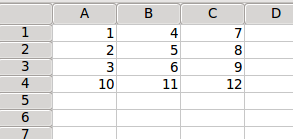
\includegraphics[width=3in]{s-data}

You can copy the values into the SAS Program Editor and save them as a file, say
\verb-x.dat-, but then you need to read them like this:

\filbreak
\begin{verbatim}
data x;
  infile 'x.dat' delimiter='09'x;
  input a b c;

proc print;

run;
\end{verbatim}
\filbreak

where the gobbledegook after \verb-delimiter- means (to SAS) that the
data values are separated by tabs, and you correctly get this output:

\filbreak
{\small
\begin{verbatim}

                                 The SAS System                               10
                                                  09:57 Monday, January 10, 2011

                             Obs     a     b     c

                              1      1     4     7
                              2      2     5     8
                              3      3     6     9
                              4     10    11    12
\end{verbatim}
}
\filbreak

If you don't put in the \verb-delimiter- part, you will get a large
number of incomprehensible error messages.

Copying {\em from} SAS might work all right for you (try it). But
since you will need to copy things from the Output window into a Word
doc (or whatever) to hand in for your assignments, let me explain what
seems to be working for me, so that you don't get stuck. To get the
above output into this document, I went to the Output window, scrolled
back a few pages (even though the bit I wanted was at the end),
selected the {\em whole window} using Edit and Select All, then I
copied it using Edit and Copy. I pasted the whole lot into my document
and then edited out the many lines that I didn't want.

The same procedure can be used to copy from the Log or even Program
Editor windows (making sure, of course, to Recall the Last Submit if
you want to copy your code).

A final remark: when you paste into your Word doc (or whatever), note
that SAS output comes in a monospaced (non-proportional) font, so it
needs to look the same way when you hand it in. A font like Courier,
or Lucida Console, is good. Also, you want to make the font small
enough so that lines don't wrap (bearing in mind that SAS output lines are
rather long). Otherwise it looks {\em really} ugly.

\end{document}
